\chapter{Obiekt symulowany - część projektowa}
Pierwszym etapem naszej pracy była analiza dostarczonego przez prowadzącego programu symulującego działanie obiektu. Był to obiekt dyskretny z opóźnieniem zależny od zmiennych procesu $U(k-11)$, $U(k-10)$, $Y(k-1)$, $Y(k-2)$.

\section{Wyznaczenie odpowiedzi skokowych procesu}
Rozpoczynając od punktu pracy $U_{\mathrm{pp}}=\num{0,8}$ i $Y_{\mathrm{pp}}=2$ wyznaczaliśmy różne odpowiedzi skokowe dla kilku zmian sygnału sterującego. Wyniki symulacji przedstawione są na Rys.~\ref{os}. Jak widać, symulowany obiekt jest stabilny (charakterystyki po pewnym czasie ustalają się na stałym poziomie) oraz liniowy (charakterystyki statyczne $Y(U)$ leżą w przybliżeniu na linii prostej, co przedstawione jest na Rys.~\ref{char_stat}).
\section{Programy do symulacji algorytmów}

Na podstawie tej charakterystyki możemy obliczyć wzmocnienie statyczne procesu. Definiuje się je jako
\begin{equation}
K=\frac{\Delta Y}{\Delta U}
\end{equation}
Parametry $\Delta Y$ i $\Delta U$ są stałe dla dowolnie wybranych punktów na wykresie $Y(U)$, ponieważ charakterystyka jest liniowa. Należy więc wybrać dowolne punkty $(U_i, Y_i)$ i $(U_j, Y_j)$ i na ich podstawie obliczyć wzmocnienie statyczne $K$. Wynik:
{\huge DO UZUPEŁNIENIA, SORY IDE NA LABY XD}

\begin{figure}
\label{os}
\centering
\caption{Odpowiedzi skokowe dla procesu symulowanego}
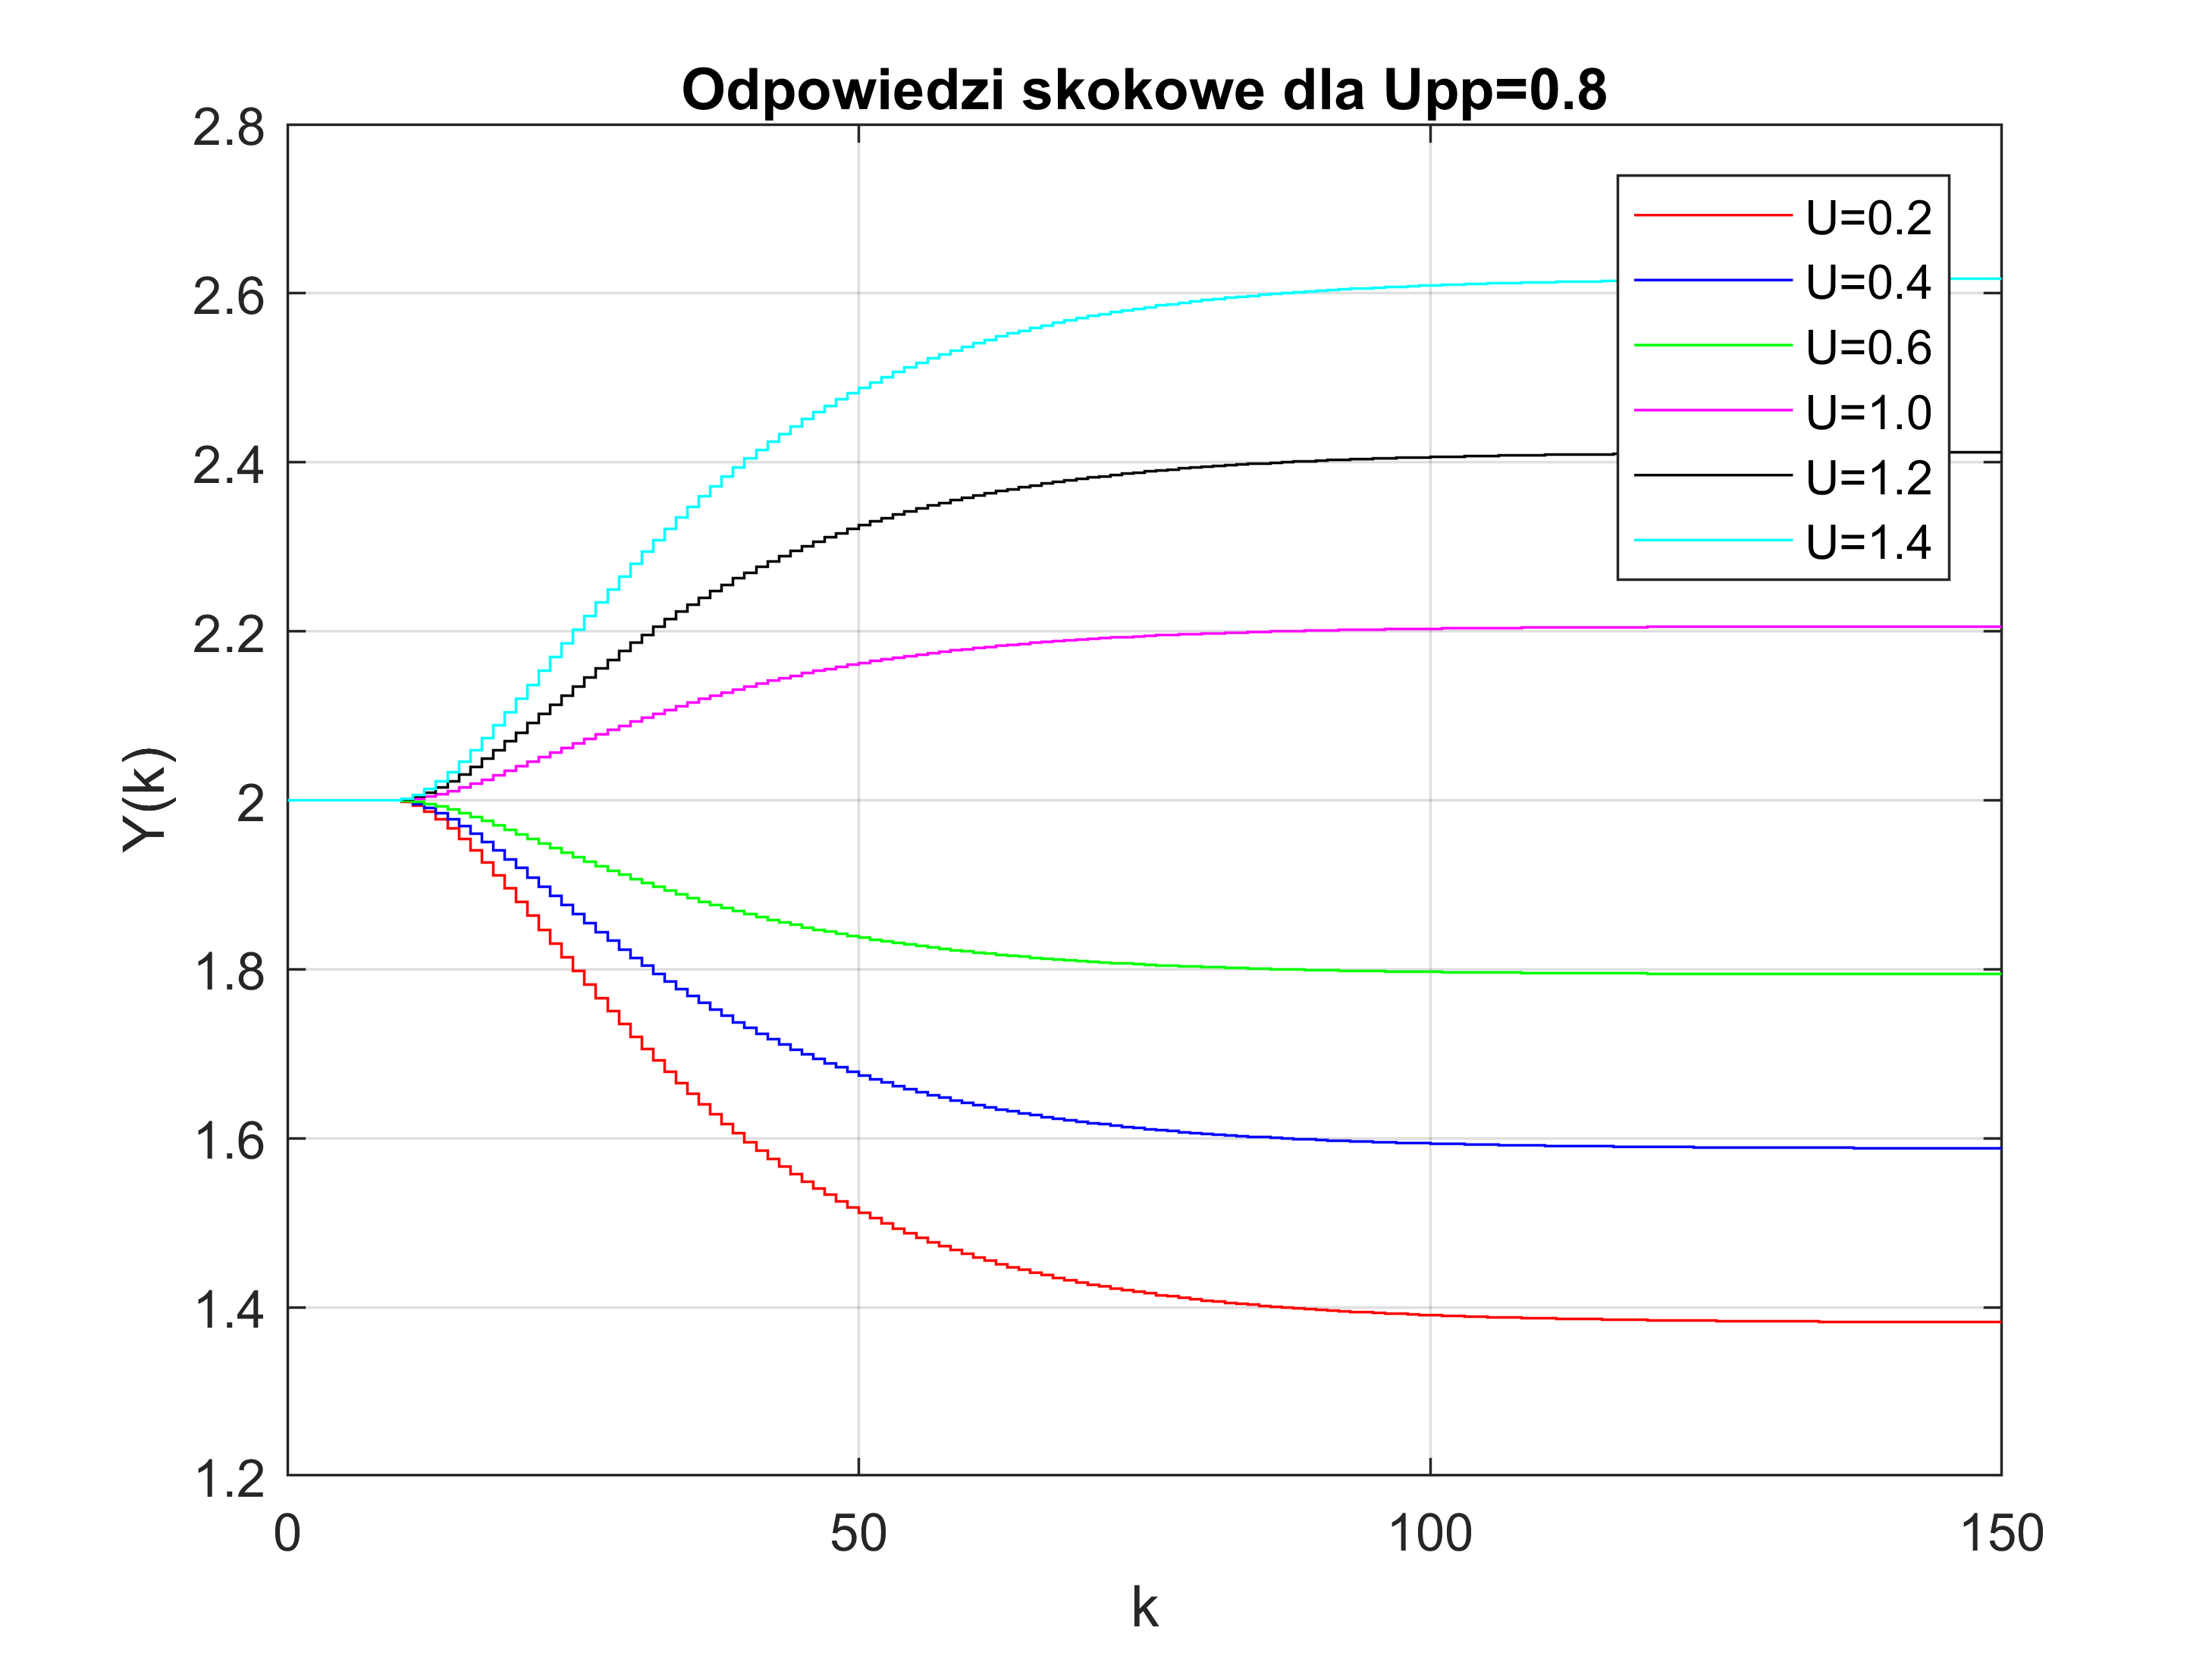
\includegraphics{odpsk.png}
\end{figure}

\begin{figure}
\label{char_stat}
\centering
\caption{Charakterystyki statyczne $Y(U)$}
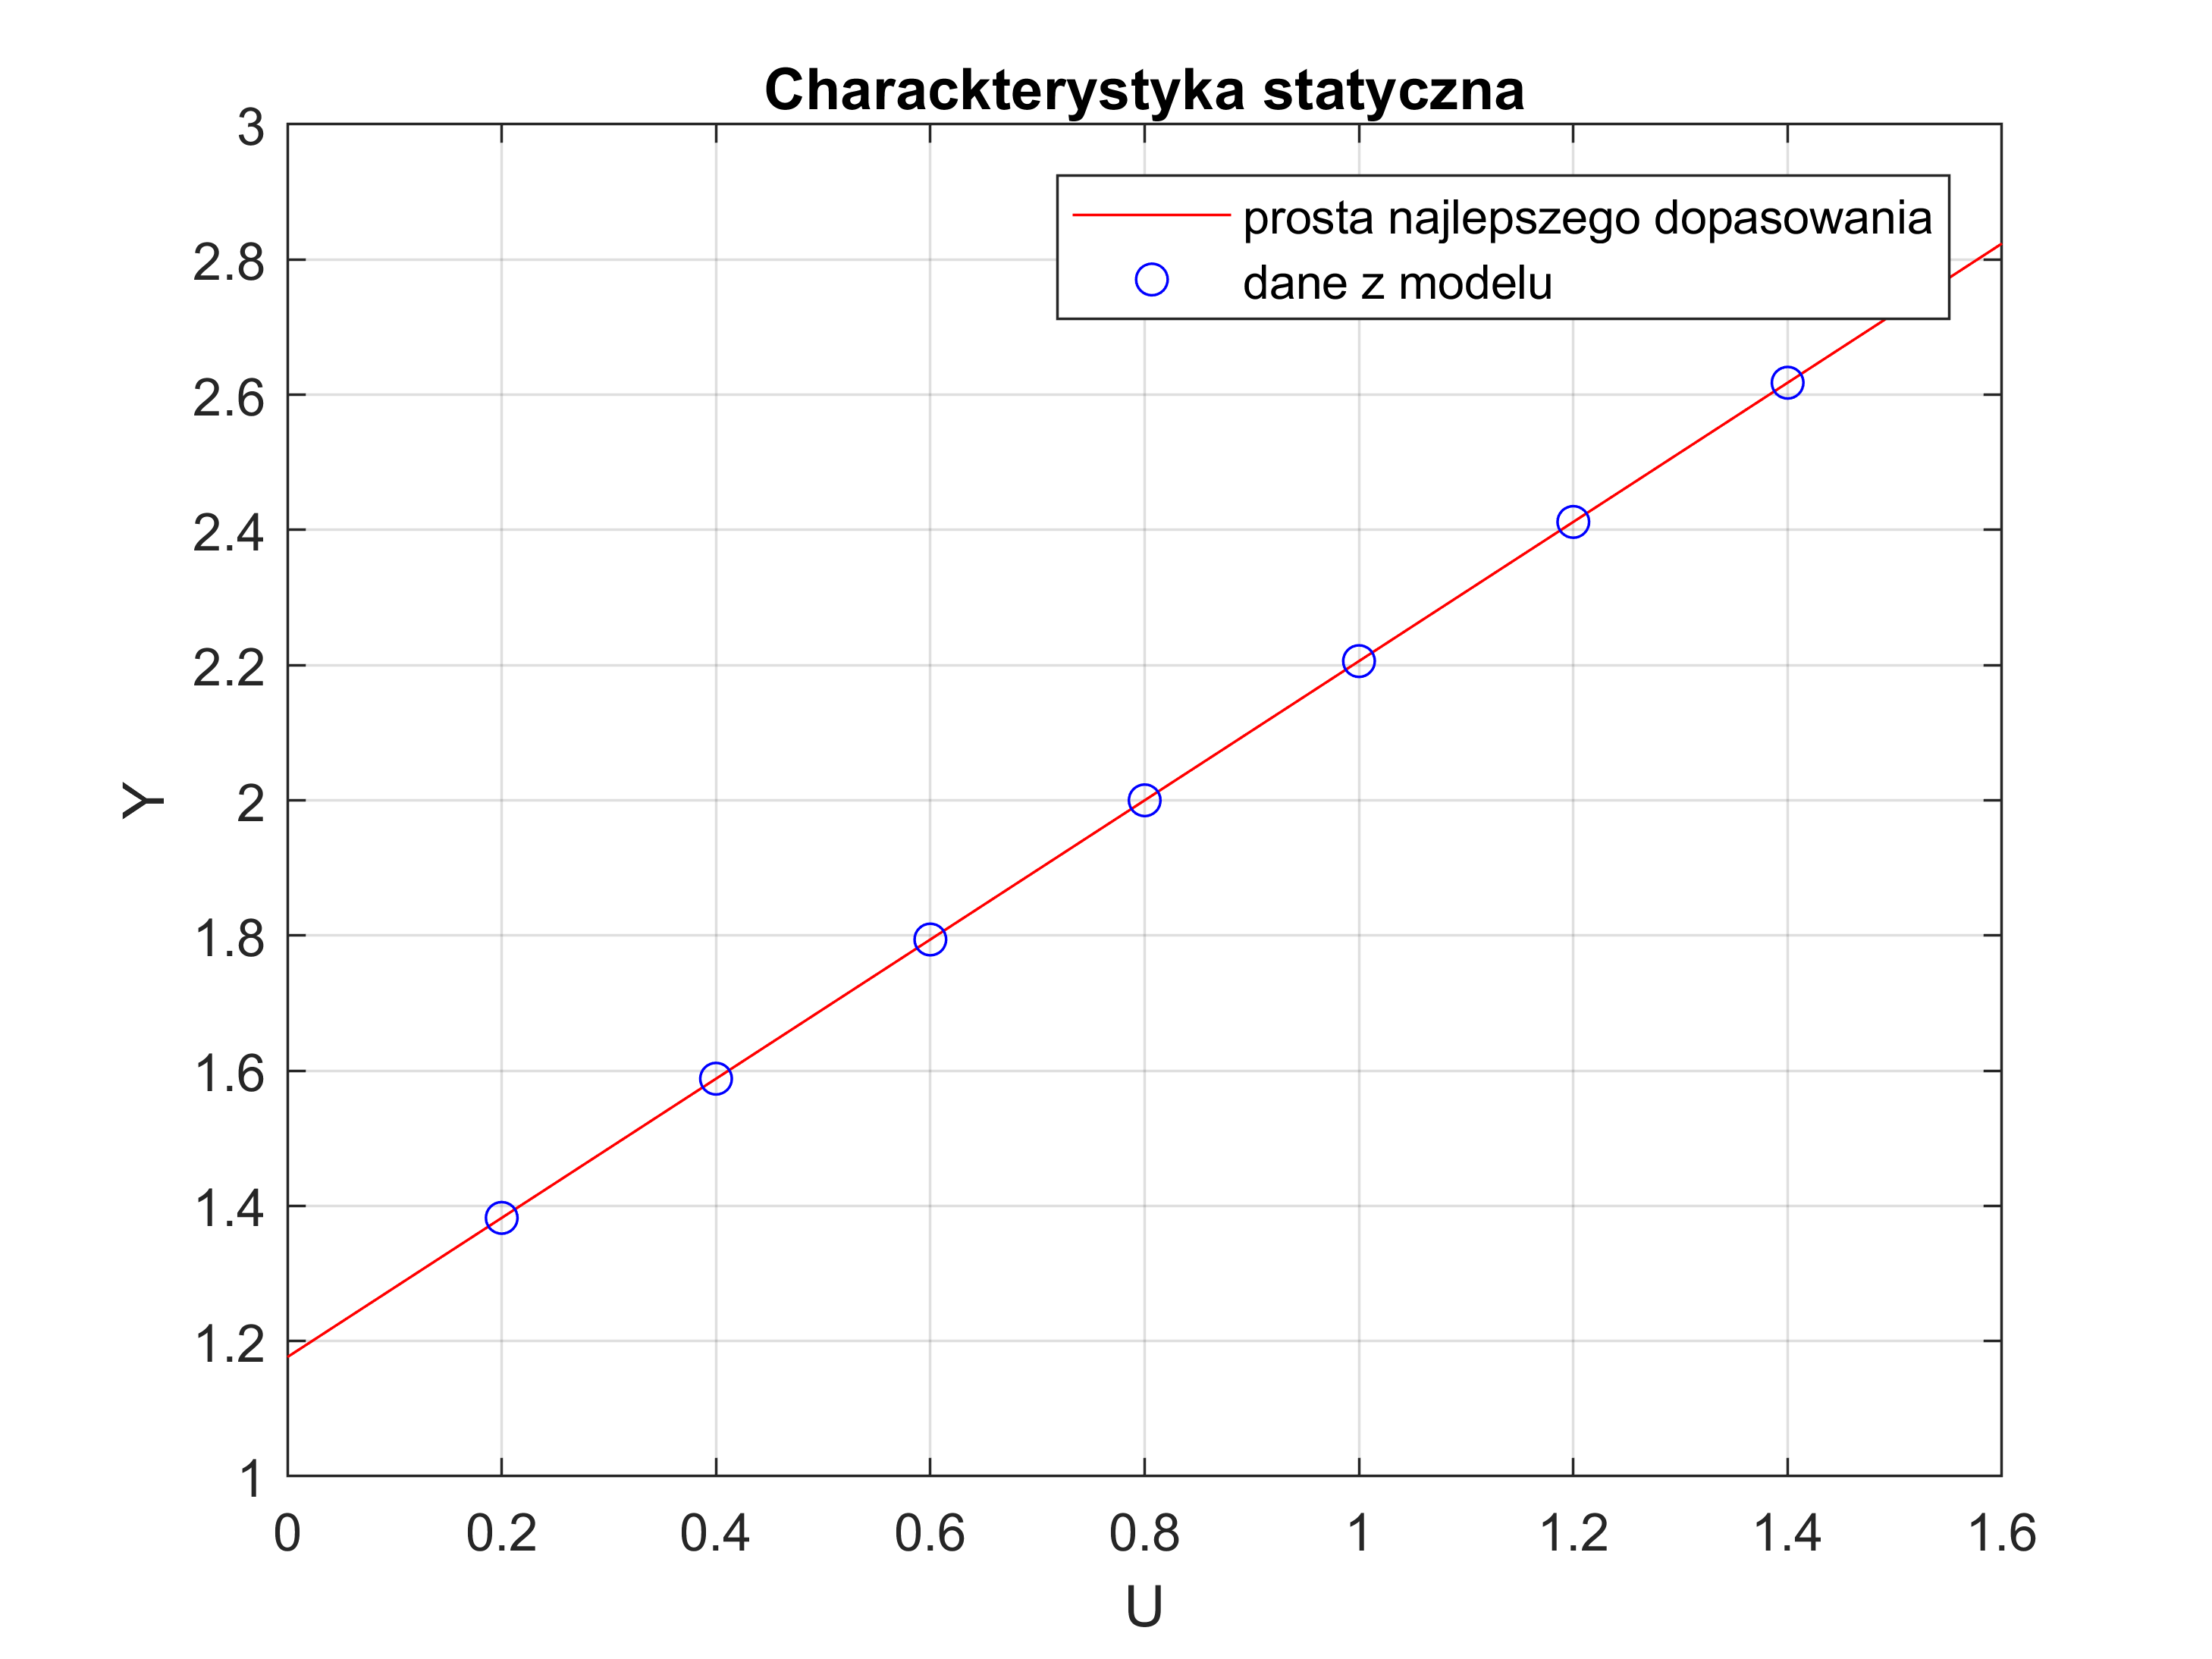
\includegraphics{static_characteristics.png}
\end{figure}

\section{Regulator PID}

\section{Algorytm DMC}

\section{Optymalizacja wskaźnika jakości}